\section{Literature review}

A vast literature exists on optimization problems where the goal is to fit a set of objects inside of one or more larger objects. Perhaps the simplest example is the knapsack problem (KP), where a set of items is defined, each with a corresponding volume and profit. A subset of items must be selected such that the sum of the profits is maximized, with the constraint that the sum of the volumes does not exceed the volume of a certain knapsack \cite{MARTELLO1987}. Mathematically, let $V \in \mathbb{R}$ be the volume of the knapsack, and $p, v \in \mathbb{R}^n$ be the vectors containing, respectively, the profit and volume associated with each item $i \in \{1,\dots,n\}$. It is possible to define a binary programming (BP) model to find out which items must be selected to solve the KP to optimality. \cref{bp1,bp2,bp3} are an example of such a problem. \cref{bp1} specifies the profit maximization problem, with $x \in \mathbb{R}^n$ being the vector of decision variables that describe whether an item is selected ($x_i = 1$) or not ($x_i = 0$). \cref{bp2} enforces that the selected items do not exceed the volume of the knapsack. \cref{bp3} specifies that vector $x$ is binary.

\begin{align}
    \min\ &p'x& \label{bp1}\\
    \text{s.t. } &\sum_{i=1}^{n}v_ix_i \leq V,&\label{bp2}\\
    &x_i \in \{0,1\},\ &\forall i \in \{1,\dots,n\}. \label{bp3}
\end{align}

Many cargo loading problems cannot be solved using a KP model due to its simplicity. For example, many 2D palletization problems require that rectangular shapes be placed on a pallet, maximizing profits while avoiding overlaps between items and respecting the rectangular boundaries of the pallet. These constraints cannot be translated into a KP, and so the model has to be extended. See, for instance, two mixed-integer optimization models proposed by \textcite{KALVELAGEN2021} to solve this type of problem. Similarly, \textcite{CHEN1995} proposed a model to load items into containers, which involves three-dimensional coordinates and even more complex enforcement of overlaps and relative positions. This is done by introducing alternative constraints to the models, which, combined with the hundreds of binary variables that are often necessary to solve the problems, makes such methods computationally unfeasible for many real applications.

The field of container loading problems (CLPs), like \cite{CHEN1995}, is vast and full of research gaps \cite{CENTENARO2024}. According to a literature review by \textcite{BORTFELDT2012}, who studied 163 papers on CLPs from 1980 to 2011, a total of ten types of constraints can be identified in the literature:

\begin{enumerate}
    \item \textbf{Weight limits:} Refer to how much weight the container can carry.
    \item \textbf{Weight distribution:} Impose weight balances, to avoid applying too much force on a specific area of the container.
    \item \textbf{Loading priorities:} Give more urgency to the placement of certain types of items, such as products that may expire soon.
    \item \textbf{Orientation:} Constrain the possible rotations of certain items. For example, fragile objects may break if rotated sideways.
    \item \textbf{Stacking:} Specify what items, and how many, may be placed on top of certain types of items.
    \item \textbf{Complete shipment:} Force subsets of items to be placed in the same container.
    \item \textbf{Allocation:} Similar to complete shipment, but also including the fact that certain groups of items may not be placed into the same container.
    \item \textbf{Positioning:} Attempt, for example, to group similar items together in a container, for easier deployment.
    \item \textbf{Stability:} Guarantee that items will not fall down (vertical stability) or violently collide with the container walls (horizontal stability).
    \item \textbf{Pattern complexity:} Attempts to make item placement simple to understand, so that human operators can more efficiently load them.
\end{enumerate}

The model presented by \cite{CHEN1995} considers only constraints 2 and 4. Yet, due to its exact nature, it is not applicable to problems with hundreds or thousands of items. For this reason, most research on CLPs has been done using inexact methods, which, according to \textcite{FANSLAU2010}, can be divided into three categories:

\begin{enumerate}[(a)]
    \item Conventional heuristics: Methods that were conceived specifically for the purpose of solving CLPs. Examples include the wall-building \cite{GEORGE1980}, layer-building \cite{BISCHOFF1995} and block-building \cite{ELEY2002} heuristics. Typically, wall-building methods divide the container into cuboid layers, resembling walls, which are successivelly filled with items by following a set of rules. Layer-building methods are similar, except for the fact that layers are built on top of one another. Block-building methods do not necessarily fill sequential spaces; rather, they search for the best current cuboid spaces to place items in, and attempt to put items of the same type adjacent to each other (thus generating blocks of items).
    \item Metaheuristics: Methods that can be adapted to solve a wide variety of problems. Generally, metaheuristics owe their flexibility to the natural processes they are based on, which can be easily abstracted. Two common examples for solving CLPs are simulated annealing \cite{EGEBLAD2009} and genetic algorithms \cite{GONÇALVES2011}. In simulated annealing, a random solution is generated and evaluated. At each iteration of the method, a slight alteration is introduced to the solution (e.g. one item takes the spot of another during the placement process), and the result of this change is evaluated. If the new solution is better, it replaces the old solution. Otherwise, there is still a chance that the new solution replaces the older one, but it decreases over time. This helps the method avoid local optima. Genetic algorithms are a more robust alternative to simulated annealing: Multiple solutions are considered at the same time, and they may be combined and modified through each iteration. Genetic algorithms are discussed in more detail in \cref{sec:GA}
    \item Tree search: Methods that create trees of possible loadings in an attempt to filter promising solutions. These include the method by \textcite{FANSLAU2010}, the improvement step of the block-building heuristic \cite{ELEY2002}, and the tree search method by \textcite{LIU2014}.
\end{enumerate}

\subsection{Genetic algorithms}\label{sec:GA}


Genetic algorithms (GAs) are brute force methods that utilize principle of natural selection to find good solutions to a problem. Initially proposed by \textcite{HOLLAND1992} in 1975, GAs have become one of the most widely used heuristics to solve a variety of optimization problems, thanks to its robustness when it comes to representing and solving problems.

The principles of natural selection were initially proposed by \textcite{DARWIN1859}, who believed that the different characteristics of individuals in a population were the key to their adaptation in a given environment. The more varied a population is, the greater the chances that at least one type of individual will prove fit to survive in its environment. Hence, the fittest individuals are more likely to live to produce offspring, and so their characteristics carry on to the next generation.

With the subsequent discoveries of chromosomes and DNA, the biological mechanisms by which individuals' traits are perpetuated in a population became clearer. It also clarified why certain individuals can possess characteristics that are drastically different to those of their progenitors -- a process known as mutation.

A chromosome is a DNA molecule that carries genetic information pertaining to an individual. It is divided into smaller sections called genes. The contents of each gene -- called alleles -- specify the different traits of a specimen. For instance, one gene may inform the eye color of an animal, while another may inform the blood type of the animal. Similarly, in a GA, chromosomes are vectorial representations of solutions to a given problem. Hence, they can be schematized like in \cref{fig:chromosome}. In this case, the alleles are the different possible values stored in each gene. Often, alleles are binary (0 or 1) \cite{KATOCH2021}; however, this is not always the case -- for certain problems, it is better to let alleles assume any natural value \cite{HERMAWANTO2013} or any value in a real interval \cite{GONÇALVES2011}.

\begin{figure}[ht]
    \centering
    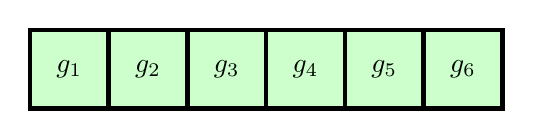
\begin{tikzpicture}
        \foreach \x in {1,...,6}
        {
            \draw[fill=green!20, ultra thick] (\x, 1.5) rectangle ++(1, 1) node[pos=.5] {$g_{\x}$};
        }
    \end{tikzpicture}
    \caption{Illustration of a chromosome with 6 genes}
    \label{fig:chromosome}
\end{figure}

It is important to define chromosomes in a way that they can be converted back into the solution that generated them. Once this is done, the next step in the GA is to define a fitness function. This function converts the chromosome back into a solution and evaluates its results. Often, the best the solution, the higher its fitness value. With the fitness function, solutions can be ranked, and thus it is possible to favor the selection of fitter chromosomes for reproduction \cite{KATOCH2021,SASTRY2005}.

With chromosomial structure and fitness function defined, the GA follows a series of steps to generate, evaluate and evolve populations with each generation \cite{SASTRY2005}:

\subsubsection*{Initialization}

    A population of $n$ solutions (chromosomes) is generated, either randomly or through a specialized method. Though $n$ is arbitrary, research indicates that if it is too small for a given problem, the GA may get stuck in a local optimum; if it is too large, it may consume more computational resources without improving the population. Different types of problems may require different population sizes, and human expertise is helpful to figure out the size to use \cite{ROEVA2013}.

 \subsubsection*{Evaluation}
 
    All solutions in the population are evaluated and ranked using the fitness function.
    
\subsubsection*{Selection}
    
    Chromosomes are selected in pairs to generate offspring in the recombination stage. One common example of selection procedure is \emph{roulette selection}, which works as follows: Suppose a population with $n \geq 2$ individuals. To each solution $i$ we associate a probability $p_i = q_i / \sum_{j=1}^{n}q_j$ of $i$ being selected. We attribute interval $I_1 = [0, p_1]$ to solution 1, and each subsequent solutions $k$ is associated with interval $I_k = \left(\sum_{j=1}^{k-1}p_j, \sum_{j=1}^{k}p_j\right]$. It results that $\cup_{j=1}^{n}I_j = [0, 1]$, so we generate a random value $r \in [0, 1]$ and pick chromosome $k$ such that $r \in I_k$ \cite{CARVALHO,SASTRY2005}. If a few solutions are much fitter than the rest, roulette selection may favor them too much and limit genetic variety early on. \emph{Ranking selection} gives value 1 to the worst solution and $n$ to the best solution, and then uses these values to generate the roulette. Thus, it can be used to more uniformly distribute the probabilities of selecting each solution. Another method that increases worse solutions' chances of selection is \emph{tournament selection}, where a subset of the population is picked, and the best chromosome from the subset is selected.

\subsubsection*{Recombination}

    Two selected parents are combined to create new chromosomes. The simplest method is \emph{one-point recombination}, and it works as follows: Suppose two parents with $m$ genes each. A point $k$ such that $1 < k < m$ is defined. The first offspring chromosome receives the first $k$ genes from the first parent and the last $m - k$ genes from the second. The same happens to the second offspring chromosome, but with the order of parents switched. This procedure can be generalized into a $k$-\emph{point recombination}, as illustrated in \cref{fig:recombination 2 points}, which shows a 2-point recombination producing two offspring.

    \begin{figure}[ht]
        \centering
        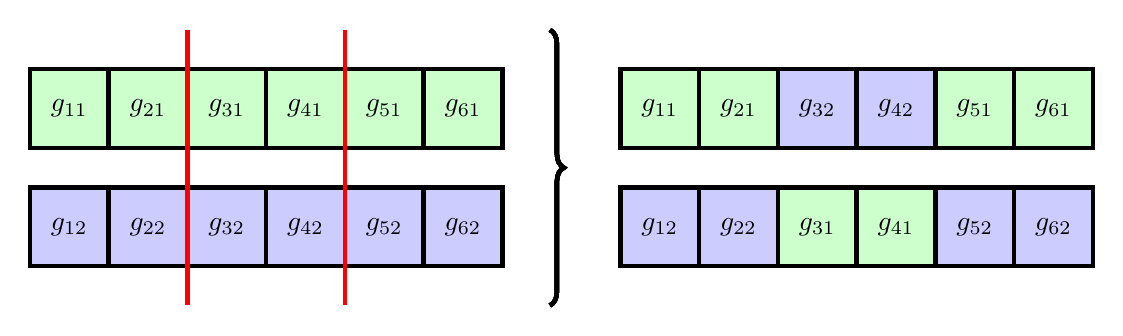
\begin{tikzpicture}
            \foreach \x in {1,...,6}
            {
                %pai 1
                \draw[fill=green!20, ultra thick] (\x, 1.5) rectangle ++(1, 1) node[pos=.5] {$g_{\x 1}$};
                %pai 2
                \draw[fill=blue!20, ultra thick] (\x, 0) rectangle ++(1, 1) node[pos=.5] {$g_{\x 2}$};
                %brace
                \draw[decorate,decoration={brace,amplitude=5pt,mirror,raise=4ex},ultra thick] (7, -0.5) -- (7, 3);
            }
            \foreach \x in {1,...,2}
            {
                %filho 1
                \draw[fill=green!20, ultra thick] (\x + 7.5, 1.5) rectangle ++(1, 1) node[pos=.5] {$g_{\x 1}$};
                \draw[fill=blue!20, ultra thick] (\x + 9.5, 1.5) rectangle ++(1, 1) node[pos=.5] {$g_{\the\numexpr\x+2 2}$};
                \draw[fill=green!20, ultra thick] (\x + 11.5, 1.5) rectangle ++(1, 1) node[pos=.5] {$g_{\the\numexpr\x+4 1}$};
                %filho 2
                \draw[fill=blue!20, ultra thick] (\x + 7.5, 0) rectangle ++(1, 1) node[pos=.5] {$g_{\x 2}$};
                \draw[fill=green!20, ultra thick] (\x + 9.5, 0) rectangle ++(1, 1) node[pos=.5] {$g_{\the\numexpr\x+2 1}$};
                \draw[fill=blue!20, ultra thick] (\x + 11.5, 0) rectangle ++(1, 1) node[pos=.5] {$g_{\the\numexpr\x+4 2}$};
            }
            \draw[color=red, ultra thick] (3, 3) -- (3, -0.5);
            \draw[color=red, ultra thick] (5, 3) -- (5, -0.5);
        \end{tikzpicture}
        \caption{2-point recombination example.}
        \label{fig:recombination 2 points}
    \end{figure}

    Another common recombination method is \emph{uniform crossover}. In this method, a binary vector (mask) is generated, with the same length as the parent chromosomes. One of the offspring takes genes from the first parent where the mask is equal to 0, or the second parent where the mask is equal to 1. The other offspring does the same, but it alternates the parent chromosomes. \cref{fig:uniform crossover} illustrates this procedure.


    \begin{figure}[ht]
        \centering
        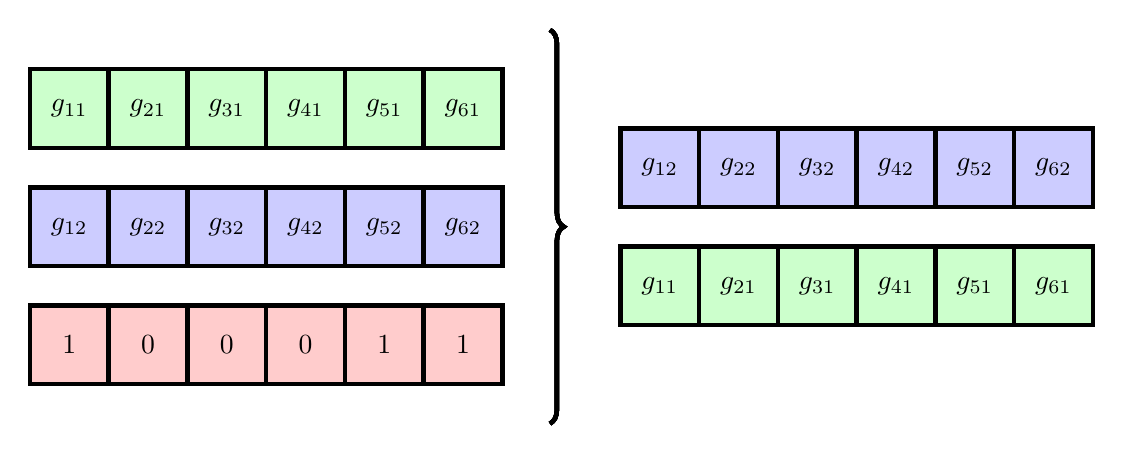
\begin{tikzpicture}
            \foreach \x/\b in {1/1,2/0,3/0,4/0,5/1,6/1}
            {
                %pai 1
                \draw[fill=green!20, ultra thick] (\x, 3) rectangle ++(1, 1) node[pos=.5] {$g_{\x 1}$};
                %pai 2
                \draw[fill=blue!20, ultra thick] (\x, 1.5) rectangle ++(1, 1) node[pos=.5] {$g_{\x 2}$};
                %máscara
                \draw[fill=red!20, ultra thick] (\x, 0) rectangle ++(1, 1) node[pos=.5] {\b};
                %brace
                \draw[decorate,decoration={brace,amplitude=5pt,mirror,raise=4ex},ultra thick] (7, -0.5) -- (7, 4.5);
                \ifthenelse{\b = 1}{\draw[fill=green!20, ultra thick] (\x + 7.5, 2.25) rectangle ++(1, 1) node[pos=.5] {$g_{\x 1}$};
                \draw[fill=blue!20, ultra thick] (\x + 7.5, 0.75) rectangle ++(1, 1) node[pos=.5] {$g_{\x 2}$};}{\draw[fill=green!20, ultra thick] (\x + 7.5, 0.75) rectangle ++(1, 1) node[pos=.5] {$g_{\x 1}$};
                \draw[fill=blue!20, ultra thick] (\x + 7.5, 2.25) rectangle ++(1, 1) node[pos=.5] {$g_{\x 2}$};}
            }
        \end{tikzpicture}
        \caption{Uniform crossover using a mask.}
        \label{fig:uniform crossover}
    \end{figure}

    $k$-point recombination consumes less resources than uniform crossover; however, the use of masks makes uniform crossover more oriented towards diversity in the next population \cite{KATOCH2021}. Furthermore, the mask can be generated in a way that gives both parents equal odds of contributing genes, or it can favor the chromosome with the better fitness value \cite{SASTRY2005}.

 \subsubsection*{Mutation}
 
    The solutions resulting from the recombination step may randomly have part of their genes changed. This is important to explore neighboring solutions and avoid convergence to local optima, if the parents are too similar. A common way of mutating chromosomes is to go through each gene and generate a number in $[0,1]$. If this number is below a probability $p$, the gene's value is replaced with a random new value \cite{SONI2014}.

\subsubsection*{Replacement}
    
    The current population is either partially or completely replaced by the offspring of the recombination and mutation processes. The GA returns to the Evaluation step, unless one or more stop criteria are reached -- for example, a certain fitness value being reached, or the maximum number of iterations.